\subsection{Method}
\subsubsection{Particle data}
The dataset used here is the \(40\)GeV simulated Higgs cascade decay used in section~\ref{sec:dataset6040}.
One Standard Model (SM) Higgs at \(125\)GeV decays to two light Higgs at \(40\)GeV,
which in turn decay to \beau{}-\bbar{} quark pairs.
That is \(H_{125\text{GeV}} \rightarrow h_{40\text{GeV}} h_{40\text{GeV}} \rightarrow \beau \bbar \beau \bbar\).


This dataset has the desirable property of creating \bthing{jets} with a range of geometries
owing to the boost provided by large mass of the SM Higgs and
the high chance of overlap with 4 \bthing{quarks} in the event.
Other radiation from the protons is also included.  % TODO clarify exactly what background is in here!


Before any evaluation can be performed on the final state of the simulation
particles that ended outside the range of the silicon tracker (\(|\eta|>2.5\))
or particles with low transverse momentum (\(p_T < 0.5\) GeV) are cut.
This is to mimic restrictions from reconstruction accuracy.

\begin{figure}[htp]
    \begin{minipage}[c]{0.5\textwidth}
        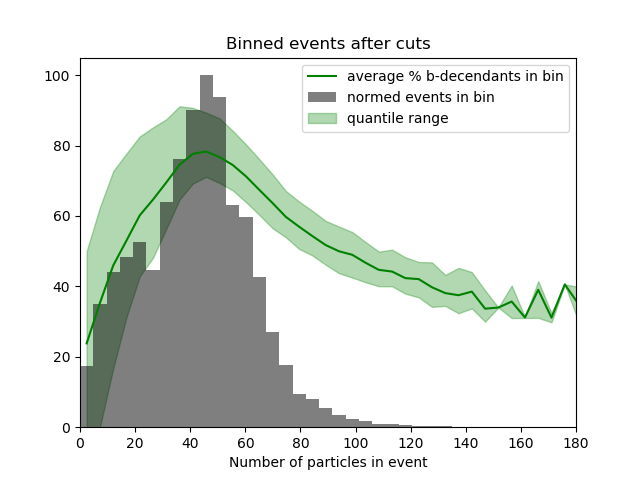
\includegraphics[width=1\textwidth]{graphics/binned_events.png}
    \end{minipage}\hfill
    \begin{minipage}[c]{0.45\textwidth}
        \caption{The end state particle in the simulated events are filtered
            with the standard cuts, \(p_T > 0.5\), \(|\eta| < 2.5\).
            The events are binned according to how many particles remain after the cuts.
            The percentage of \bthing{descendants} in the remaining event after the cuts
            is averaged for each bin and plotted on the same axis.
            After the cuts have been applied most events are left with around \(50\) particles.
                 The percentage of particles that are descendant from a \bthing{quark} varies,
                 it is at it's highest in events with \(50\) particles,
             and most variable in events will small multiplicity.}\label{fig:bdecendantpercent}
    \end{minipage}
\end{figure}    

A particle is considered a \bthing{descendant} if is found in the chain of decays from a \bthing{quark}.
After cuts, \(72\%\) of events have at least \(5\) \bthing{descendants} and \(5\) non \bthing{descendants} available.
Exactly how the percentage of \bthing{descendants} changes with event size is visualised in figure~\ref{fig:bdecendantpercent}.

\subsubsection{Clustering algorithm}\label{sec:spectralmethodalgo}
Now the implementation of the theory described in section~\ref{sec:spectral_theory} will be specified.
For every simulated event this process if used to select a clustering.

\begin{enumerate}
    \item \label{step:start} The particles are to be used to form the nodes of a graph,
    the edges of which will be weighted by some measure of proximity between the particles known as affinity.
    To obtain an affinity, first a distance is obtained; \(d_{i,j} = \sqrt{(y_i - y_j)^2 + (\phi_i - \phi_j)^2}\)
    where \(y_i\) is the rapidity of particle \(i\) and \(\phi_i\) is the barrel angle is particle \(i\).

    \item The affinity must increase as particles become more similar, whereas the distance will shrink.
        This is done by taking an exponent so that \(a_{i,j} = \text{exp}(2d_{i,j})\).%, as done in~\cite{hadjighasem2016votex}. % TODO check you stick with this

    \item These affinities allow the construction of a Laplacian.
    The Laplacian used is the unnormalised Laplacien, which has \(\sum_j a_{i,j}\) in the \(i\)th
    diagonal entry (also known as the degree of node \(i\)) and \(-a_{i,j}\) of the diagonal 
    in column \(i\) row \(j\).

    \item From the Laplacian a predetermined number of eigenvectors are calculated to create the embedding space.
    The eigenvectors have as many elements as there are particles, and the coordinates of
    the \(i\)th particle in the embedding space is the \(i\)th element of each eigenvector.

    \item The first clustering can be done based on 
    a measure of distance derived from the particles \(p_T\) and its position in the embedding space.
    The \(p_T\) is used as in the Luclus~\cite{moretti1998new}, with a variable exponent, \(q\);
    \[p_T \text{ factor} = \left(\frac{{p_T}_i{p_T}_j}{s({p_T}_i+{p_T}_j)}\right)^q.\]
    Where \(s\) is the invariant mass of all observed particles in the event, it is used
    to make the \(p_T\) factor unitless.
    The embedded distance is euclidean distance in the embedding space multiplied by this factor.

    \item The two objects that have the smallest embedding distance are combined.
    In physical space the combined object is created by summing the respective four momenta,
    in the embedding space two methods for locating the combined object are tried.
    \begin{enumerate}
        \item In a \spectralmeanjet{} clustering the location of the combined object is the
        geometric mean of the inputs. The clustering then continues to combine things in this manner.
        \item In a \spectralfulljet{} once two object have been combined in physical space
            the embedding space is recalculated from step~\ref{step:start}. 
    \end{enumerate}

    \item When the closest object to a particle in the embedding space is further away than \stoppingdeltar{}
    then the combined object is considered to be a complete jet and removed from future clustering.
\end{enumerate}
To provide a basis for comparison the results of clustering with an anti-kt algorithm (as in~\cite{Cacciari2008akt}) is also shown.

